%////////////////////////////////////////////////////////////////////////////////////////////////////////////
% INSTITUTO TECNOLOGICO DE COSTA RICA
% Escuela de Ingenieria en Construccion
% Construction Engineering School
% https://www.tec.ac.cr
% Eng. MSc. Maikel Mendez Morales
% Email: maikel.mendez@gmail.com; mamendez@itcr.ac.cr
% https://orcid.org/0000-0003-1919-141X
% https://www.scopus.com/authid/detail.uri?authorId=51665581300
% https://scholar.google.com/citations?user=JnmSVFYAAAAJ&hl=en
% https://www.youtube.com/c/maikelmendez
% https://twitter.com/MaikelMendezM
% https://github.com/maikelonu
% Skype: maikel.mendez
%////////////////////////////////////////////////////////////////////////////////////////////////////////////

%-------------------------------------------------------------------------------------------------------------------
% INFO: This script is intended as a LATEX template for class "Laboratorio de Hidraulica CO-3503"
%-------------------------------------------------------------------------------------------------------------------

%/////////////////////////////////////////////////////////////////////////////////////////////////////////////
% BLOCK: LATEX document configuration and packages loading
%/////////////////////////////////////////////////////////////////////////////////////////////////////////////

% Sheet format and letter size is defined
\documentclass[12pt, letterpaper]{article} 

% Margens are defined
\usepackage[left=2cm,right=2cm,top=3cm,bottom=3cm]{geometry} 

%Translates various standard and input encodings into LaTeX internal language
\usepackage[utf8]{inputenc} 

% Several mathematical symbolologies are defined
\usepackage{amsmath} 
\usepackage{amsfonts} 
\usepackage{amssymb}

% Mathematical equations are enumerated
\usepackage{makeidx}

% Document language is selected
\usepackage[spanish]{babel}

% Document spacing is defined
\usepackage{setspace}

% Document spacing is set
\onehalfspacing %Spacing

% Improves interface for floating objects (figures and tables)
\usepackage{float} 

% Allows manipulation of images, headers, footers, etc.
\usepackage{graphicx}

% Bibliography packages are loaded
\usepackage[backend=bibtex]{biblatex}

% References (*.BIB) file is loaded !!!
\addbibresource{reference.bib}

% Allows adding references within the index
\usepackage[nottoc]{tocbibind} 

%/////////////////////////////////////////////////////////////////////////////////////////////////////////////
% BLOCK: LATEX document writing
%/////////////////////////////////////////////////////////////////////////////////////////////////////////////

% Document is started
\begin{document}
%---------------
-------------------------------------------------------------------
% Title page is created manually
\begin{titlepage}
%----------------------------------------------------------------------------------

% TEC's logo is added
% This is used to center the text
\begin{center} 

\begin{figure}[H]
	\centering
	
\includegraphics[width=1\columnwidth]{LOGO_TEC.png}
\end{figure}

   %This command makes the letter bigger and bold.
	\textbf{\large{ESCUELA DE INGENIERÍA EN CONSTRUCCIÓN}}\\
	\textbf{\large{LABORATORIO DE HIDRÁULICA}}\\
	\textbf{\large{Grupo 3}} \\

\vspace{1in} % This command sets a space between lines.
\textbf{\large{INFORME 4. VISCOSIDAD CINEMÁTICA}}\\
\vspace{1in}
\textbf{\large{Elaborado por:}}\\
\textbf{\large{ALEJANDRA TREJOS ELIZONDO  CARNÉ}}\\
\textbf{\large{DANIELA MAROTO CALDERÓN  CARNÉ}}\\
\vspace{0.5in}
\textbf{\large{Profesor guía:}}\\
\textbf{\large{MAIKEL MÉNDEZ MORALES}}\\
\vspace{0.5in}
\textbf{\large{Fecha de entrega:}}\\
\textbf{\large{19 de setiembre}}\\
\vspace{1in}
\textbf{\large{II Semestre 2017}}\\

\end{center}

\end{titlepage}

%----------------------------------------------------------------------------------
% Table of contents is created
\tableofcontents
%----------------------------------------------------------------------------------

% A pagebreak is added
\pagebreak

%----------------------------------------------------------------------------------
% Resumen section is created
\section{RESUMEN}
%----------------------------------------------------------------------------------

El siguiente informe muestra las actividades realizadas en un experimento dirigido a analizar la viscosidad cinemática de un fluido en el que se evalua la concordancia entre dos columnas capilares, una $N^{\circ}300$ y otra $N^{\circ}150$. El principal objetivo del informe es medir las viscosidades con dos instrumentos diferentes y analizar si existe concordancia en los resultados.\\
El fluido que se utilizó fue un aceite SAE 20W-50, se determinó su viscosidad a distintas temperaturas que van desde los $30^{\circ}C$ hasta los $115^{\circ}C$. Una vez obtenidos los resultados, se introdujeron a R Studio, donde se analizó la concordancia de los instrumentos. Se utilizaron pruebas como Agreement para determinar concordancia y calidad de los datos, ggplot2 para generar gráficos, cor.test para determinar la correlación de datos, entre otros.\\
Para las columnas 150A y 150B el valor de TDI fue de 0,98 y un CP de 0,982, para las 300A y 300B fue de 1,318 y 0,765, respectivamente. La tolerancia de TDI fue de 1 y el CP fue de 90\%. Por lo tanto, las columnas 150 se pueden sustituir entre sí pero las 300 no. Se obtuvo una relación de la viscosidad en función de la temperatura de tipo potencial. El modelo que se logró ajustar al mismo fue $V(csT)= (3,64E\times10^{5} \pm 5,11E\times10^{4}) \times T^{(-2,11 \pm 0,0392)}$, además el coeficiente de determinación para dicho modelo es de 0,996.\\ 
Para mejorar los resultados se debe procurar la limpieza de las columnas capilares para evitar la obstrucción del flujo, evitar la estratificación de la temperatura en el fluido en este caso glicerina, entre otras posibles fuentes de error.

%----------------------------------------------------------------------------------
% Metodologia section is created
\section{METODOLOGÍA}
%----------------------------------------------------------------------------------

La siguiente metodología presenta la secuencia de cálculos ligados al experimento “Viscosidad cinemática”, en un orden secuencial, esto para diferentes columnas capilares a distintos valores de temperatura.

\subsection{Equipo utilizado}
\begin{itemize}
    \item Calentador a temperatura constante Cannon H1-A.
    \item Columnas capilares Cannon-Fenske $N^{\circ}150$. Modelo: M964 y N104.
    \item Columnas capilares Cannon-Fenske $N^{\circ}300$. Modelo: G587 y G592
    \item Aceite para motor SAE 20W-50: Marca: Pennzoil.
    \item Cronómetro. Marca: Casio, Precisión: $\pm$0,01 s.
\end{itemize}

\subsection{Conversión de unidades}
Se utiliza la siguiente conversión, la cual se extrajo del script proporcionado por el profesor.

\begin{equation}
\label{ec1}
1 cSt = 1 mm^{2}/s = 1\times10^{6} m^{2}/s
\end{equation}

\subsection{Memoria de cálculo}

El profesor proporcionó los datos utilizados un total de 6 tiempos por medida, los cuales se promediaron con la siguiente ecuación:

\begin{equation}
\label{ec2}
Promedio = \frac{Lecturas}{Total \> de \> lecturas}
\end{equation}

Además, se realizaron un total de 22 medidas con las columnas capilares dependiendo del modelo, específicamente 4 medidas para cada modelo de la columna capilar $N^{\circ}300$ y 7 medidas para cada modelo de la columna capilar $N^{\circ}150$. Estos valores dependen de las variaciones en la temperatura, para cada modelo se cuenta con una constante K, sin embargo solo se tienen los valores a $40^{\circ}C$ y $100^{\circ}C$, por lo que fue necesario interpolar y extrapolar para conocer el valor de K a la temperatura indicada, esto se realizó con la ecuación \ref{ec3}:

\begin{equation}
\label{ec3}
\frac{(100^{\circ}C - Temperatura)}{(Temperatura - 40^{\circ}C)} = \frac{(Constante \> a \> 100^{\circ}C -Constante \> K)}{(Constante \> K - Constante \> a \> 40^{\circ}C)}
\end{equation}

Al conocer los valores de temperatura y el tiempo promedio se realizó el cálculo de la viscosidad cinemática con la siguiente ecuación:
\begin{equation}
\label{ec4}
v = constante \> K\cdot t
\end{equation}
 
Donde:\\ 
v = Viscosidad cinemática (cSt)\\
constante K = Constante de viscosidad (cSt/s)\\ 
t = tiempo (s)

%----------------------------------------------------------------------------------
% Descripcion y Analisis Estadistico section is created
\section{DESCRIPCIÓN Y ANÁLISIS ESTÁDISTICO}
%----------------------------------------------------------------------------------

Para el análisis estadístico del experimento se utilizó el programa R Studio \cite{rstudio}, en él se ejecutaron las siguientes funciones que serán representadas de la siguiente manera:

\begin{enumerate}
    \item agreement {Agreement}: Esta función se encarga de computar funciones que permiten evaluar la concordancia y calidad de los datos mediante algunas pruebas; entre ellas se encuentran: concordance correlation coefficient (CCC), precision, accuracy, total deviation index (TDI), coverage probability (CP) y relative biased square (RBS).
    \item cor.test {stats}: Esta función permite asociar a dos variables independientes.
    \item Desc {DescTools}: Esta función permite crear resúmenes de varios tipos de variables; asimismo calcula estadísticas descriptivas que permiten obtener salidas numéricas y gráficas.
    \item ggplot{ggplot2}: Esta función permite la creación de gráficas tipo listas.
    \item nls: Realiza el cálculo de intervalos de confianza y de ajuste para un modelo no lineal.
\end{enumerate}

%----------------------------------------------------------------------------------
% Resultados section is created
\section{RESULTADOS}
%----------------------------------------------------------------------------------

A continuación se presentan los resultados del experimento “Medición de viscosidad cinemática” para un aceita SAE 20W-50 en distintas columnas capilares para verificar la correlación de los mismos.\\
Existen una serie de factores que afectan los resultados obtenidos, entre ellos se pueden mencionar la estratificación térmica, debido a que a pesar de que se hace circular la glicerina para mantener la temperatura constante, no hay manera de asegurar su distribución uniforme; también se debe mencionar el error del operario en cuanto al tiempo de reacción para la toma de tiempo y la contaminación del fluido debido a la exposición de las columnas al ambiente.\\
Así mismo, el fluido se contamina debido a que absorbe humedad del ambiente y este se emulsifica. En ciertos casos se origina la formación de burbuja, la cual es otra fuente de incertidumbre debido a que obstruye el flujo del fluido.

% **********************************************************************************
% To insert a table, you have to export it from R Studio and then paste it
% In R:
% require(xtable)
% print(xtable(nombre de la tabla), include.rownames = FALSE)
% **********************************************************************************

% **********************************************************************************
% Those of you who rather work tables in MS-EXCEL or LibreOffice, 
% should watch this tutorial: 
% [LaTeX/Excel] Excel2Latex: Conversor de Tablas de Excel a LaTeX
% https://www.youtube.com/watch?time_continue=2&v=7Eg10VOzyqw
% **********************************************************************************

\begin{table}[ht]
\centering
\begin{tabular}{rrrlll}
  \hline
temp\_C & viscosity\_m2\_s & viscosity\_cSt & column & group & fluid \\ 
  \hline
 30 & 0.00 & 276.49 & 300\_A & TECNICO & SAE\_20W50 \\ 
   40 & 0.00 & 164.49 & 300\_A & TECNICO & SAE\_20W50 \\ 
   50 & 0.00 & 99.83 & 300\_A & TECNICO & SAE\_20W50 \\ 
   60 & 0.00 & 67.50 & 300\_A & TECNICO & SAE\_20W50 \\ 
   70 & 0.00 & 44.04 & 150\_A & TECNICO & SAE\_20W50 \\ 
   80 & 0.00 & 31.49 & 150\_A & TECNICO & SAE\_20W50 \\ 
   90 & 0.00 & 23.46 & 150\_A & TECNICO & SAE\_20W50 \\ 
  100 & 0.00 & 17.93 & 150\_A & TECNICO & SAE\_20W50 \\ 
  105 & 0.00 & 15.52 & 150\_A & TECNICO & SAE\_20W50 \\ 
  110 & 0.00 & 13.83 & 150\_A & TECNICO & SAE\_20W50 \\ 
  115 & 0.00 & 12.39 & 150\_A & TECNICO & SAE\_20W50 \\ 
   30 & 0.00 & 276.81 & 300\_B & TECNICO & SAE\_20W50 \\ 
   40 & 0.00 & 165.01 & 300\_B & TECNICO & SAE\_20W50 \\ 
   50 & 0.00 & 100.75 & 300\_B & TECNICO & SAE\_20W50 \\ 
   60 & 0.00 & 68.34 & 300\_B & TECNICO & SAE\_20W50 \\ 
   70 & 0.00 & 44.90 & 150\_B & TECNICO & SAE\_20W50 \\ 
   80 & 0.00 & 32.15 & 150\_B & TECNICO & SAE\_20W50 \\ 
   90 & 0.00 & 24.03 & 150\_B & TECNICO & SAE\_20W50 \\ 
  100 & 0.00 & 18.38 & 150\_B & TECNICO & SAE\_20W50 \\ 
  105 & 0.00 & 15.93 & 150\_B & TECNICO & SAE\_20W50 \\ 
  110 & 0.00 & 14.20 & 150\_B & TECNICO & SAE\_20W50 \\ 
  115 & 0.00 & 12.74 & 150\_B & TECNICO & SAE\_20W50 \\ 
   \hline
\end{tabular}
\end{table}

\begin{table}[ht]
\centering
\caption{Set de datos de viscosidades con línea de mejor ajuste e intervales de confianza.}
\begin{tabular}{p{1.8cm}|p{1.5cm}p{1.5cm}p{1.5cm}p{1.5cm}p{2cm}p{1.2cm}p{1.2cm}p{1.2cm}}
  \hline
Temperatura ($^{\circ}C$) & Viscosidad ($m^{2}/s$) & Viscosidad (cSt) & Columna Capilar  & Grupo & Fluido & Ajuste & Inferior & Superior \\ 
  \hline
  30 & 2.80E-04 & 276.49 & 300\_A & TECNICO & SAE\_20W50 & 282.01 & 274.61 & 289.42 \\ 
  40 & 1.60E-04 & 164.49 & 300\_A & TECNICO & SAE\_20W50 & 153.86 & 150.08 & 157.63 \\ 
  50 & 1.00E-04 & 99.83 & 300\_A & TECNICO & SAE\_20W50 & 96.16 & 92.70 & 99.62 \\ 
  60 & 7.00E-05 & 67.50 & 300\_A & TECNICO & SAE\_20W50 & 65.50 & 62.32 & 68.68 \\ 
  70 & 4.00E-05 & 44.04 & 150\_A & TECNICO & SAE\_20W50 & 47.34 & 44.50 & 50.18 \\ 
  80 & 3.00E-05 & 31.49 & 150\_A & TECNICO & SAE\_20W50 & 35.73 & 33.22 & 38.24 \\ 
  90 & 2.00E-05 & 23.46 & 150\_A & TECNICO & SAE\_20W50 & 27.88 & 25.67 & 30.10 \\ 
  100 & 2.00E-05 & 17.93 & 150\_A & TECNICO & SAE\_20W50 & 22.33 & 20.37 & 24.29 \\ 
  105 & 2.00E-05 & 15.52 & 150\_A & TECNICO & SAE\_20W50 & 20.15 & 18.30 & 22.00 \\ 
  110 & 1.00E-05 & 13.83 & 150\_A & TECNICO & SAE\_20W50 & 18.27 & 16.53 & 20.01 \\ 
  115 & 1.00E-05 & 12.39 & 150\_A & TECNICO & SAE\_20W50 & 16.64 & 14.99 & 18.28 \\ 
  30 & 2.80E-04 & 276.81 & 300\_B & TECNICO & SAE\_20W50 & 282.01 & 274.61 & 289.42 \\ 
  40 & 1.70E-04 & 165.01 & 300\_B & TECNICO & SAE\_20W50 & 153.86 & 150.08 & 157.63 \\ 
  50 & 1.00E-04 & 100.75 & 300\_B & TECNICO & SAE\_20W50 & 96.16 & 92.70 & 99.62 \\ 
  60 & 7.00E-05 & 68.34 & 300\_B & TECNICO & SAE\_20W50 & 65.50 & 62.32 & 68.68 \\ 
  70 & 4.00E-05 & 44.90 & 150\_B & TECNICO & SAE\_20W50 & 47.34 & 44.50 & 50.18 \\ 
  80 & 3.00E-05 & 32.15 & 150\_B & TECNICO & SAE\_20W50 & 35.73 & 33.22 & 38.24 \\ 
  90 & 2.00E-05 & 24.03 & 150\_B & TECNICO & SAE\_20W50 & 27.88 & 25.67 & 30.10 \\ 
  100 & 2.00E-05 & 18.38 & 150\_B & TECNICO & SAE\_20W50 & 22.33 & 20.37 & 24.29 \\ 
  105 & 2.00E-05 & 15.93 & 150\_B & TECNICO & SAE\_20W50 & 20.15 & 18.30 & 22.00 \\ 
  110 & 1.00E-05 & 14.20 & 150\_B & TECNICO & SAE\_20W50 & 18.27 & 16.53 & 20.01 \\ 
  115 & 1.00E-05 & 12.74 & 150\_B & TECNICO & SAE\_20W50 & 16.64 & 14.99 & 18.28 \\ 
   \hline
\end{tabular}\\
Fuente: R Studio, a partir de los datos brindados por el profesor Maikel Méndez.
\end{table}

\begin{table}[ht]
\centering
\caption{Resultados del modelo no lineal planteado.}
\begin{tabular}{ccccc}
  \hline
Parámetro & Desviación estándar & Error & t-Value  & Pr-Value \\ 
  \hline
  a & 3.64E+04 & 5.11E+04 & 7.126 & 6.63E-07*** \\ 
  Power & -2.11E+00 & 3.92E-02 & -53.712 & -2.00E-02*** \\ 
  \hline
\end{tabular}\\
Fuente: R Studio, a partir de los datos brindados por el profesor Maikel Méndez.
\end{table}

\begin{table}[ht]
\centering
\caption{Ecuación y coeficiente de determinación del comportamiento de la viscosidad con respecto a la temperatura.}
\begin{tabular}{cc}
  \hline
Ecuación & $V=3.643x10^{5}\cdot T^{-2.11}$ \\ 
  \hline
  $R^{2}$ & 0.996 \\ 
   \hline
\end{tabular}\\
Fuente: R Studio, a partir de los datos brindados por el profesor Maikel Méndez.
\end{table}


\begin{table}[ht]
\centering
\caption{Set de datos de viscosidades obtenidas mediante las columnas 150A y 150B con sus respectivas desviaciones simples.}
\begin{tabular}{cccc}
  \hline
ID & Columna 150A & Columna 150B & Desviación Simple \\ 
  \hline
  1 & 44.04 & 44.90 & 0.86 \\ 
  2 & 31.49 & 32.15 & 0.66 \\ 
  3 & 23.46 & 24.03 & 0.57 \\ 
  4 & 17.93 & 18.38 & 0.45 \\ 
  5 & 15.52 & 15.93 & 0.41 \\ 
  6 & 13.83 & 14.20 & 0.37 \\ 
  7 & 12.39 & 12.74 & 0.35 \\ 
   \hline
\end{tabular}\\
Fuente: R Studio, a partir de los datos brindados por el profesor Maikel Méndez.
\end{table}

\begin{table}[ht]
\centering
\caption{Resultados de la prueba agreement para las columnas 150A y 150B.}
\begin{tabular}{cccccc}
  \hline
Valores & CCC & Precisión & Exactitud & TDI & CP \\ 
  \hline
  Resultados & 0.999 & 0.999 & 0.980 & 0.980 & 0.982 \\ 
  Tolerancia & 0.975 & - & - & 1.000 & 0.900 \\ 
   \hline
\end{tabular}\\
Fuente: R Studio, a partir de los datos brindados por el profesor Maikel Méndez.
\end{table}

\begin{table}[ht]
\centering
\caption{Set de datos de viscosidades obtenidas mediante las columnas 300A y 300B con sus respectivas desviaciones simples.}
\begin{tabular}{cccc}
  \hline
ID & Columna 300A & Columna 300B & Desviación Simple \\ 
  \hline
  1 & 276.49 & 276.81 & 0.32 \\ 
  2 & 164.49 & 165.01 & 0.52 \\ 
  3 & 99.83 & 100.75 & 0.92 \\ 
  4 & 67.50 & 68.34 & 0.84 \\ 
   \hline
\end{tabular}\\
Fuente: R Studio, a partir de los datos brindados por el profesor Maikel Méndez.
\end{table}

\begin{table}[ht]
\centering
\caption{Resultados de la prueba agreement para las columnas 300A y 300B.}
\begin{tabular}{cccccc}
  \hline
Valores & CCC & Precisión & Exactitud & TDI & CP \\ 
  \hline
  Resultados & 1.000 & 1.000 & 1.000 & 1.318 & 0.764 \\ 
  Tolerancia & 0.975 & - & - & 1.000 & 0.900 \\ 
   \hline
\end{tabular}\\
Fuente: R Studio, a partir de los datos brindados por el profesor Maikel Méndez.
\end{table}

\begin{table}[ht]
\centering
\caption{Resultados de las medias de la desviación simple para las columnas 300 y 150.}
\begin{tabular}{ccccc}
  \hline
Desviación Simple & Columna 150 & Columna 300 \\ 
  \hline
  Media & 0.524 & 0.650
  \\ 
  \hline
\end{tabular}\\
Fuente: R Studio, a partir de los datos brindados por el profesor Maikel Méndez.
\end{table}

\begin{landscape}

\begin{figure}[H]
	\centering
	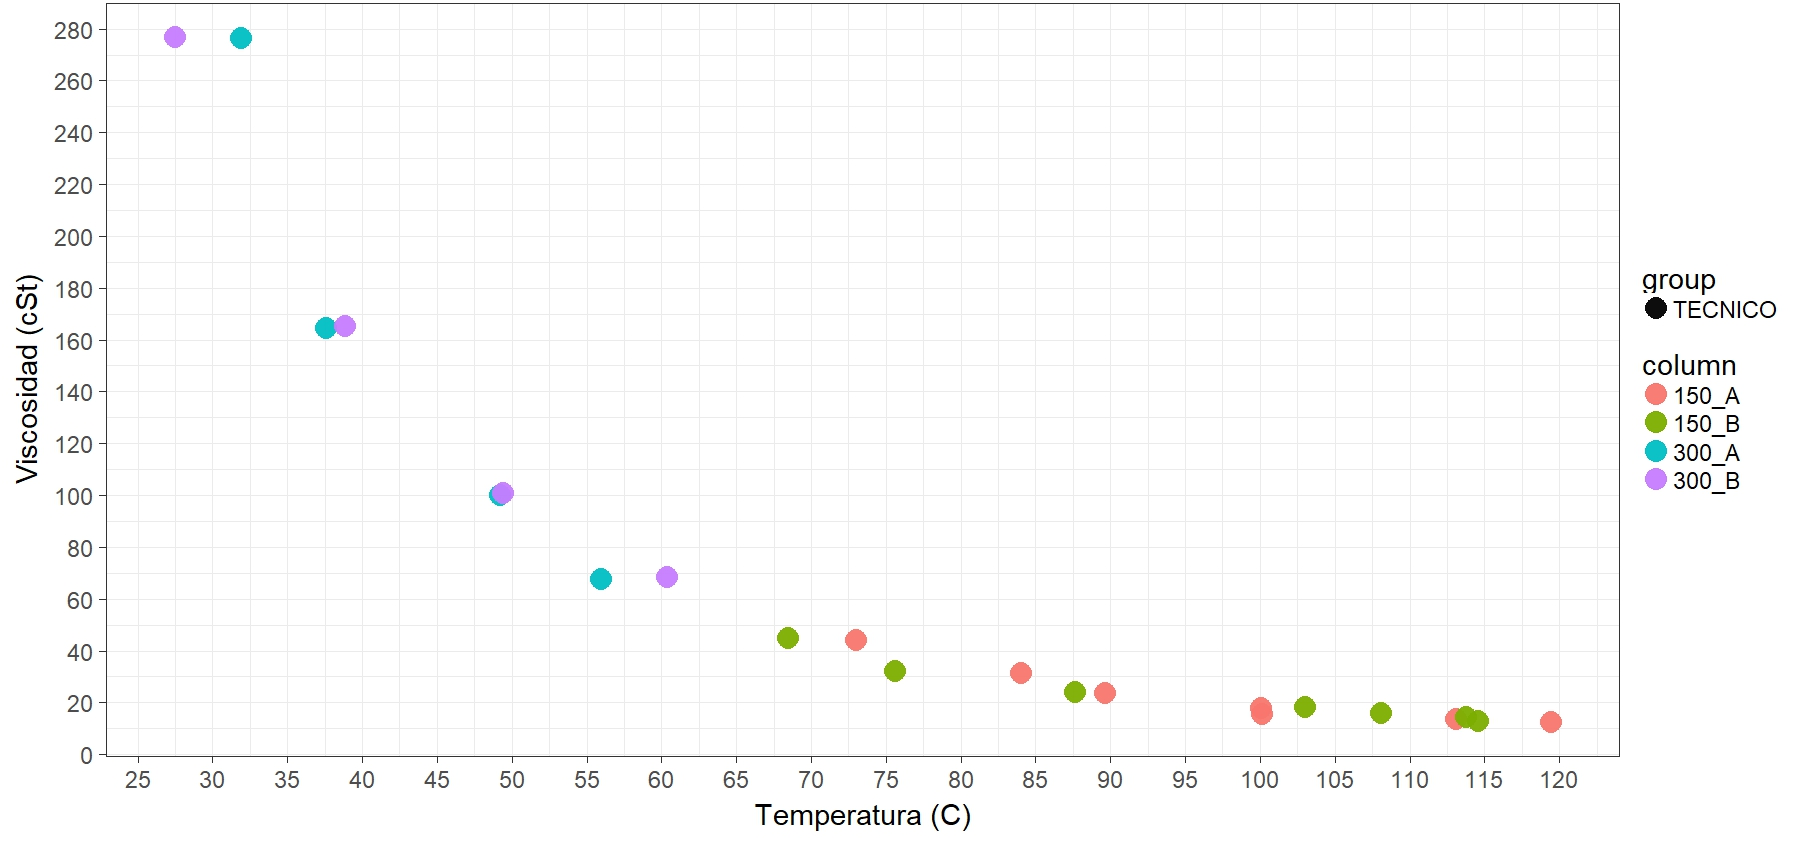
\includegraphics[width=1\columnwidth]{figura_1.png}
	\caption{Valor de viscosidad (cSt) en función de la temperatura ($^{\circ}C$).}
	Fuente: R Studio, a partir de los datos del cuadro 1.
    \label{figura1}
\end{figure}

\begin{figure}[H]
	\centering
	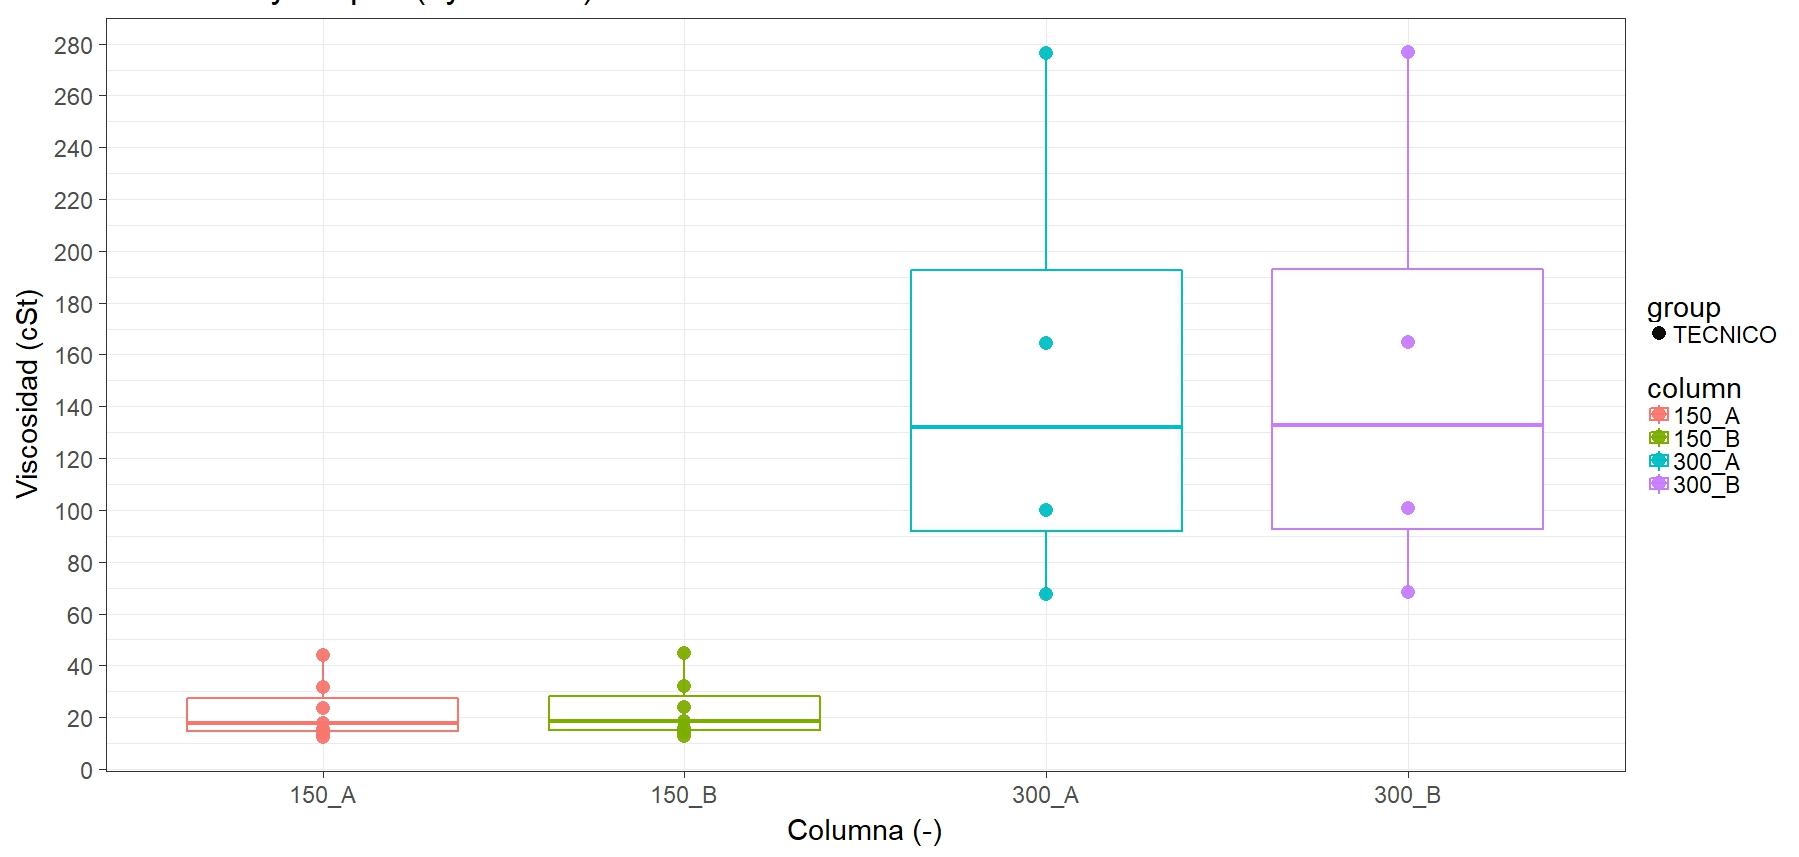
\includegraphics[width=1\columnwidth]{figura_2.png}
	\caption{Valor de viscosidad (cSt) por columnas capilares}
    Fuente: R Studio, a partir de los datos del cuadro 1.
    \label{figura2}
\end{figure}

\begin{figure}[H]
	\centering
	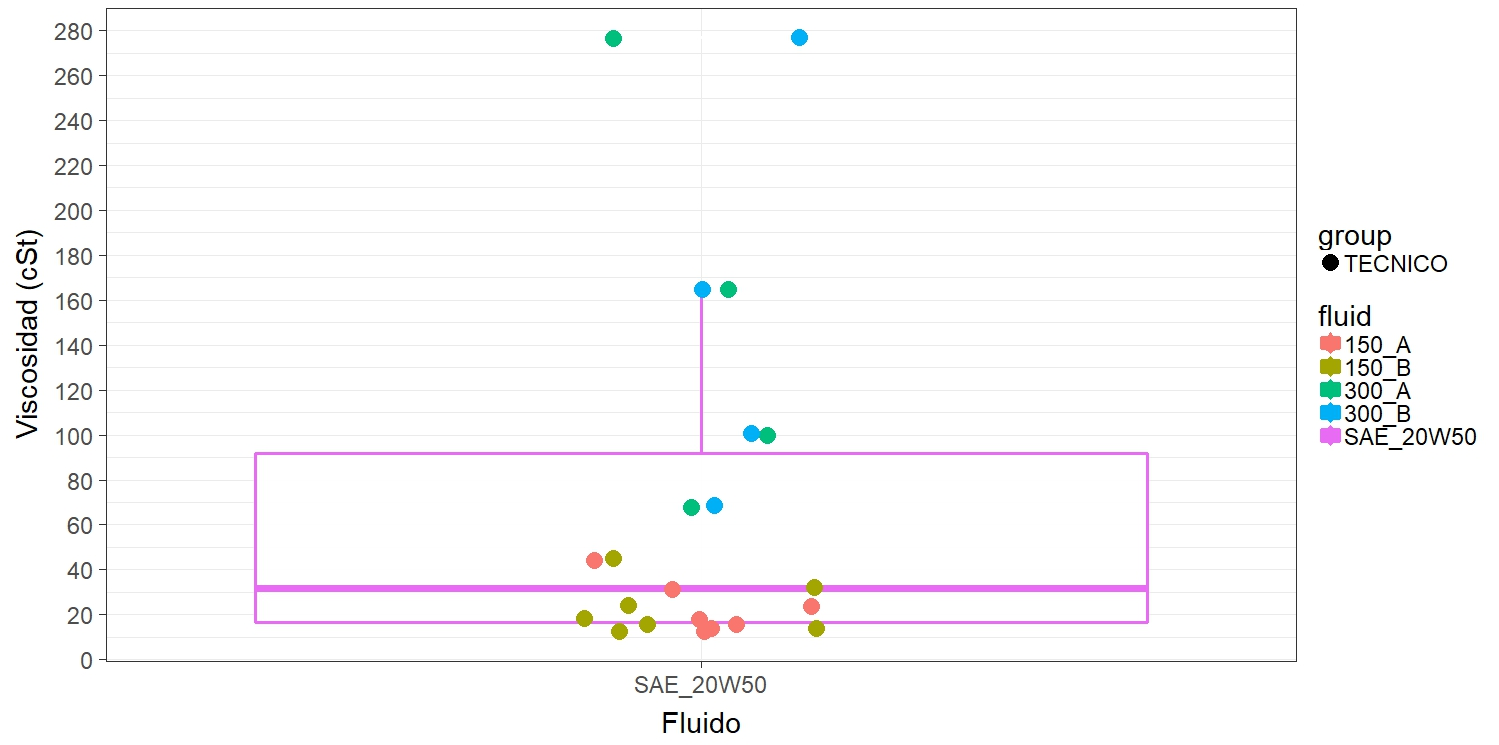
\includegraphics[width=1\columnwidth]{figura_3.png}
	\caption{Valor de viscosidad (cSt) en función del fluido.}
	Fuente: R Studio, a partir de los datos del cuadro 1.
    \label{figura3}
\end{figure}

\begin{figure}[H]
	\centering
	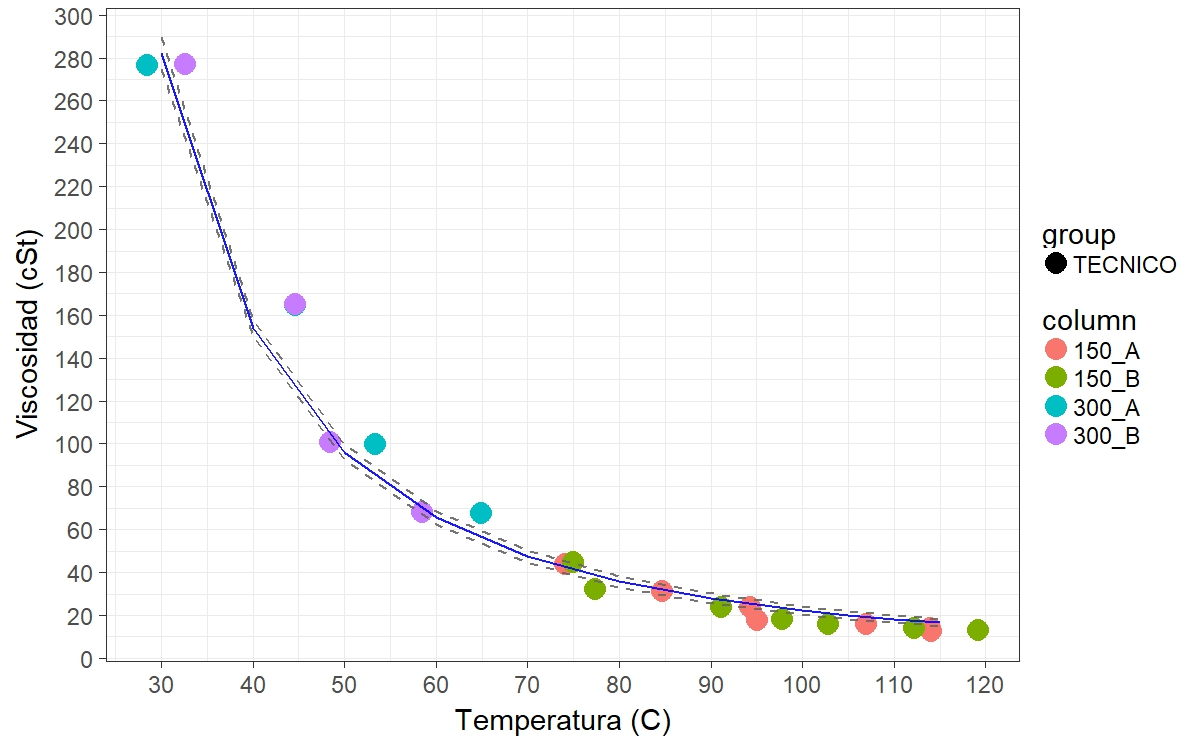
\includegraphics[width=1\columnwidth]{figura_4.png}
	\caption{Valor de viscosidad (cSt) en función de la temperatura ($^{\circ}C$) con línea de mejor ajuste.}
	Fuente: R Studio, a partir de los datos del cuadro 1.
    \label{figura4}
\end{figure}

\begin{figure}[H]
	\centering
	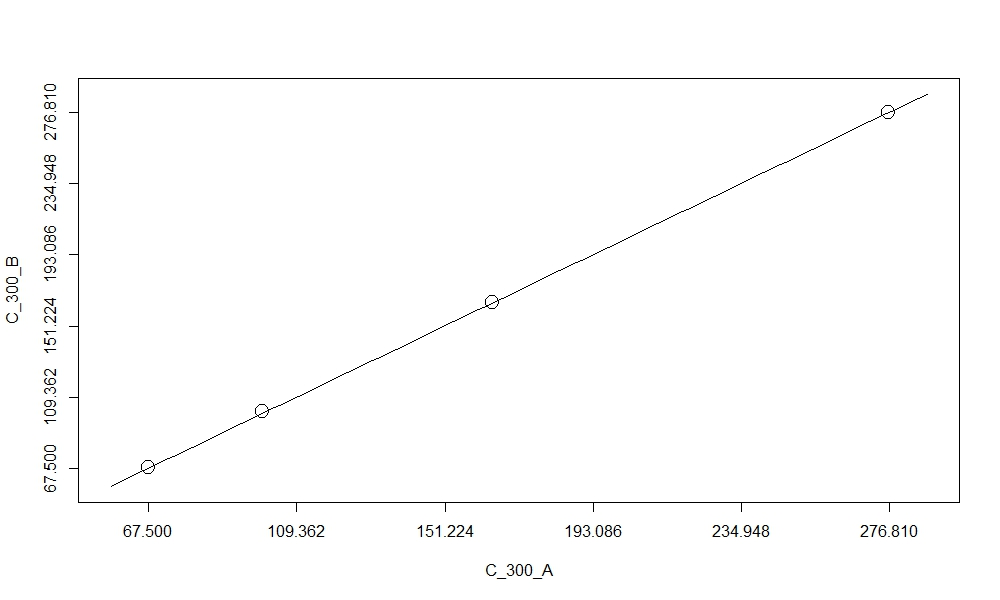
\includegraphics[width=1\columnwidth]{figura_5.png}
	\caption{Análisis gráfico de la concordancia entre los datos tomados con las dos columnas 300.}
	Fuente: R Studio, a partir de los datos del cuadro 6.
    \label{figura5}
\end{figure}

\begin{figure}[H]
	\centering
	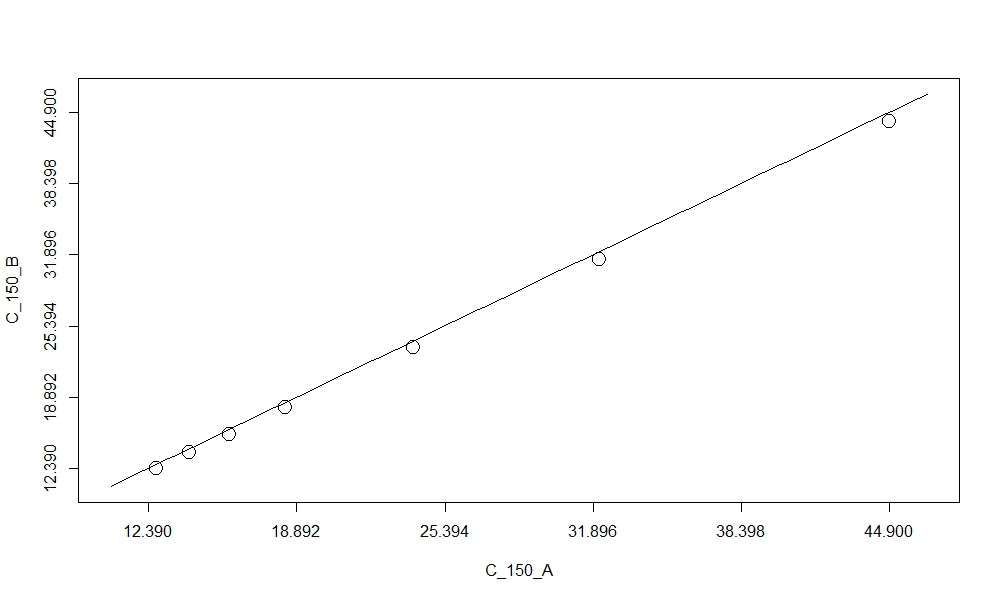
\includegraphics[width=1\columnwidth]{figura_6.png}
	\caption{Análisis gráfico de la concordancia entre los datos tomados con las dos columnas 150.}
	Fuente: R Studio, a partir de los datos del cuadro 4.
    \label{figura6}
\end{figure}

\end{landscape}

%----------------------------------------------------------------------------------
% Analisis de Resultados section is created
\section{ANÁLISIS DE RESULTADOS}
%----------------------------------------------------------------------------------

En este informe se pretende conocer la relación de la viscosidad cinemática de un fluido respecto a su temperatura. Según el ingeniero \cite{marcano}, la viscosidad  expresa la facilidad que tiene un fluido para fluir cuando se le aplica una fuerza externa; por lo tanto es una medida de su resistencia al deslizamiento o a la deformación cortante o angular.  Dicha medida puede obtenerse en el laboratorio, y la viscosidad se puede presentar como viscosidad dinámica o absoluta y como  viscosidad cinemática. Además; dicha resistencia que se opone al movimiento relativo de la moléculas del fluido que presenta viscosidad es gracias a la fricción cinemática. \cite{mott}. Durante el desarrollo de este análisis se estará trabajando con la viscosidad cinemática, la cual corresponde a según Mott al cociente de la viscosidad dinámica del fluido analizado y su densidad.\\
Como se mencionó al inicio del informe el objetivo principal del experimento es la comparación de las viscosidades entre el mismo tipo de columnas; así como la dependencia de la temperatura en dichos valores.\\ 
En el cuadro 1 se muestra los datos de las viscosidades experimentales tomadas por el técnico Heiner Navarro Mena, para las columnas capilares de 150 y 300 del tipo Cannon Fensk; las cuáles son seleccionadas según el rango de temperatura en que se necesite trabajar. Como se observa se tomaron mediciones para dos columnas de cada tipo, cabe destacar que dichas columnas presentan el mismo modelo, pero distinto número de serie y son utilizadas para medir temperaturas en un rango de $30^{\circ}C$ a $60^{\circ}C$ y de $70^{\circ}C$ a $115^{\circ}C$. Las mismas presentan con constantes de calibración diferentes que se obtienen en cada una de sus fichas técnicas.\\ 
Como se debía de medir el tiempo que tardaba el fluido en pasar entre dos marcas de la columna, una de las posibles fuente de error es el tiempo de reacción y percepción que presentaba la persona encargada de las mediciones.\\
Se puede en los resultados experimentales del cuadro 1, la relación de dependencia de la viscosidad respecto a la temperatura; dicha relación se observa gráficamente en la figura 1; en donde se muestra que a medida que se aumente la temperatura, la viscosidad empieza a disminuir sus valores; es decir hay una relación inversamente proporcional de la viscosidad respecto a la temperatura, es decir hay una relación decreciente no lineal para estas variables.\\
Se muestra además en la figura \ref{figura2}, el comportamiento de las mediciones según la columna utilizada. Se esperaba que mediante esta figura se pudiera observar una misma viscosidad para cada uno de los modelos de columnas; ya que cada una de las series fueron trabajadas a mismas temperaturas; y el equipo al estar bien calibrado no debería de presentar diferencias entre las medidas tomadas. Tal como se observa en la figura 2 tanto el modelo 300 A y B, como la 150 A y B presentan comportamientos muy similares y el valor de las medianas están prácticamente en el mismo nivel, lo cual era el resultado que se esperaba; debido a que la calibración del equipo no tenía que  influir en los resultados ya que sin importar cuál constante de calibración que se estuviera utilizando la viscosidad a una misma temperatura debería de ser la misma.\\ 
Asimismo se grafica otro boxplot generalizado donde se muestran los valores del comportamiento de las viscosidades en forma general, dichos resultados se observan en el figura \ref{figura3}. Como se evidencia en dicha figura, a medida que aumenta la viscosidad existe un aumento en la dispersión de los datos, tal y como se observa en el cuarto cuartil; en donde inclusive existen 2 datos atípicos correspondientes a la columna de 300. Sin embargo para la columna de 150, se observa que a medida que los valores de viscosidad son menores la dispersión de los datos disminuye. Dicha situación también se observa en la figura \ref{figura1}, en la cual se observa una variación de viscosidad menor conforme aumenta la temperatura; por el comportamiento asintótico que es registrado en el modelo potencial.\\ 
Precisamente, debido a la correlación que se ha observado hasta ahora respecto a la viscosidad y a la temperatura, es que se procede a buscar el modelo que logre representar dicha relación; por lo que se procede a regresionar la viscosidad contra la temperatura, respecto a una potencia y un coeficiente “a”. Dichos parámetros son mostrados en el cuadro 2. Se observa que el error para ambos variables es de al menos un orden de magnitud menor, lo que representa un buen primer indicador; asimismo, cuando se compara el valor del Pr-value, se nota que es menor a 0,05; lo que permite rechazar la hipótesis nula y en consecuencia se puede indicar un buen comportamiento de los datos. Asimismo se observa una significancia de 3 asteriscos; lo cual es la condición más alta de significancia. Además se realiza una prueba de correlación entre las variables, dicho resultado se muestra en el cuadro 3 y se observa que el valor obtenido del coeficiente de determinación es de 0,996; lo cual muestra la existencia de una buena predicción con el modelo potencial.\\ 
Además en el cuadro 1 se muestra el resultado del valor ajustado del modelo, que se obtuvo mediante la función predict; así como los intervalos de confianza superior e inferior. Dichos valores se representan gráficamente en la figura \ref{figura4}, en dicha figura se puede observar la comparación entre las viscosidades medidas en el laboratorio respecto a la viscosidad del modelo potencial, con los intervalos de confianza mostrados en el cuadro 1. Las líneas punteadas de la figura representan los límites superior e inferior de confianza; y se puede observar que existen zonas donde el modelo potencial presenta puntos angulares; ya que en estos rangos no existen muchas mediciones. Como se puede observar, las columnas de 150 son utilizadas en rangos donde se requiera una mayor temperatura; a diferencia de las columnas de 300 que son utilizadas en temperaturas más bajas.\\ 
Para realizar un análisis entre la concordancia de las series de cada uno de los modelos de las columnas, se aplica la prueba agreement para conocer si los instrumentos son equivalentes y se puede reemplazar la columna A por la columna B.En el cuadro 8 se observa los valores de las medias obtenidas para ambos modelos, y su valor se encuentra por debajo del valor meta establecido; lo cual representa un buen indicativo de las diferencias entre las series de las columnas.\\
En el cuadro 4, se muestra una comparación de los datos experimentales de las viscosidades obtenidas para el modelo de la columna 150, además su desviación estándar; en el cuadro 6 se muestra los mismo datos de las desviaciones estándar pero para la columna de 300. Con dichos resultados se procede a realizar el análisis de la prueba agreement para ambas columnas, los resultados de la columnas de 150 son mostradas en el cuadro 5. Se observa que el valor del CCC (0,9987) es mayor a la tolerancia de 0,975; lo cual indica que el producto entre la precisión y la exactitud es bastante aceptable, afirmando que estos instrumentos son bastante precisos y exactos. Asimismo se definió un valor meta o TDI de 1 y un CP del 90\%. Para esta columna de 150 se obtuvo que el 0,9082 de las observaciones se encuentran en un rango de desviación del 0,98; lo cual es menor al error esperado; indicando que para este caso, las distintas series de la misma columna pueden ser reemplazadas una con la otra. 
Se realiza la misma prueba agreement, pero para las columnas de 300. Dichos resultados son mostrados en el cuadro 7. Se observa un valor de CCC de 1; lo cual muestra relaciones de precision y exactitud perfectos, sin embargo se muestra que el valor del CP se encuentra por debajo de la tolerancia del 90\% de los datos dentro del error establecido; en este caso se obtuvo que un 0,7646 de los datos se encuentran en un rango de error mayor a la desviación establecida como meta la cual era de 1. Por lo tanto para el caso de las columnas de 300, no se puede indicar que las distintas series del mismo modelo puedan ser reemplazadas las unas con la otras.\\ 
Los resultados de la prueba agreement se pueden observar de mejor forma en las figuras \ref{figura5} y \ref{figura6}. Para las columnas de 150 se observa en la figura \ref{figura6}, como todos los puntos se encuentran de forma muy cercana a la línea ideal de $45^{\circ}$; indicando la relación existente entre los datos de cada serie. Mientras que para los datos de la columna de 300, se observa en la figura \ref{figura4} mayores desviaciones, lo cual también se puede observar en el cuadro 6.\\ 
Es importante destacar las fuentes de error que pudieron afectar a los resultados; las mismas según lo mencionado por el profesor Maikel Méndez en clases, corresponden a el estado de limpieza las columnas, ya que la contaminación ambiental puede perjudicar al aceite, el cual tiende a absorber humedad y provocar emulsificación del mismo; la emulsificación según \cite{chow}, hace referencia a la formación de fases líquidas inmiscibles, una de las cuáles se dispersa a través de la otra en forma de gotas muy pequeñas, es decir es la formación de una  emulsión del líquido. Asimismo, se debe de tener en las mejores condiciones controladas la temperatura, ya que esta temperatura del medio debe de ser constante en la realización del experimento \cite{coleparmer}; además de que se debe de verificar que el fluido se encuentre en equilibrio con el medio; por lo que se debe de sumergir la columna junto con el fluido cierta cantidad de tiempo, antes de iniciar el proceso de succión.\\

%----------------------------------------------------------------------------------
% % Conclusiones section is created
\section{CONCLUSIONES}
%----------------------------------------------------------------------------------

\begin{enumerate}
    \item La viscosidad cinemática de un fluido tiende a variar respecto a los cambios de temperatura, tal y como se mostró en los resultados los cuáles fueron determinados usando viscosímetros capilares. 
    \item La relación de la viscocidad en función de la temperatura es del tipo potencial. El modelo que se logró ajustar al mismo fue el de$V(csT)= (3,64E\times10^{5} \pm 5,11E\times10^{4}) \times T^{(-2,11 \pm 0,0392)}$, además el coeficiente de determinación para dicho modelo es de 0,996.
    \item Ambos modelos de las columnas son precisos y exactos; sin embargo sólo ambas series del modelo 150 son sustituibles, a diferencia de las series del modelo 300, cuyos valores no cumplen con los límites de concordancia establecidos.
\end{enumerate}

%----------------------------------------------------------------------------------
% % Recomendaciones section is created
\section{RECOMENDACIONES}
%----------------------------------------------------------------------------------

\begin{itemize}
    \item Realizar nuevas mediciones para las viscosidades medidas con las columnas del modelo 300.
    \item Procurar la limpieza de los viscosímetros para evitar posibles fuentes de error.
    \item Asegurar que la temperatura del viscosímetro sea constante durante la ejecución del experimento.
    \item Evitar la estratificación de la temperatura en la columna.
\end{itemize}

%----------------------------------------------------------------------------------
% % Referencias section is created
\section{REFERENCIAS BIBLIOGRÁFICAS}
%----------------------------------------------------------------------------------

\printbibliography

% //////////////////////////////////////////////////////////////////////////////////
% BLOCK: EXAMPLE of a table imported from R
% //////////////////////////////////////////////////////////////////////////////////

\begin{table}[ht]
\centering
\begin{tabular}{rrrlllrrr}
  \hline
temp\_C & viscosity\_m2\_s & viscosity\_cSt & column & group & fluid & fit & lwr & upr \\ 
  \hline
30.00 & 0.00 & 276.49 & 300\_A & TECNICO & SAE\_20W50 & 282.01 & 274.61 & 289.42 \\ 
  40.00 & 0.00 & 164.49 & 300\_A & TECNICO & SAE\_20W50 & 153.86 & 150.08 & 157.63 \\ 
  50.00 & 0.00 & 99.83 & 300\_A & TECNICO & SAE\_20W50 & 96.16 & 92.70 & 99.62 \\ 
  60.00 & 0.00 & 67.50 & 300\_A & TECNICO & SAE\_20W50 & 65.50 & 62.32 & 68.68 \\ 
  70.00 & 0.00 & 44.04 & 150\_A & TECNICO & SAE\_20W50 & 47.34 & 44.50 & 50.18 \\ 
  80.00 & 0.00 & 31.49 & 150\_A & TECNICO & SAE\_20W50 & 35.73 & 33.22 & 38.24 \\ 
  90.00 & 0.00 & 23.46 & 150\_A & TECNICO & SAE\_20W50 & 27.88 & 25.67 & 30.10 \\ 
  100.00 & 0.00 & 17.93 & 150\_A & TECNICO & SAE\_20W50 & 22.33 & 20.37 & 24.29 \\ 
  105.00 & 0.00 & 15.52 & 150\_A & TECNICO & SAE\_20W50 & 20.15 & 18.30 & 22.00 \\ 
  110.00 & 0.00 & 13.83 & 150\_A & TECNICO & SAE\_20W50 & 18.27 & 16.53 & 20.01 \\ 
  115.00 & 0.00 & 12.39 & 150\_A & TECNICO & SAE\_20W50 & 16.64 & 14.99 & 18.28 \\ 
  30.00 & 0.00 & 276.81 & 300\_B & TECNICO & SAE\_20W50 & 282.01 & 274.61 & 289.42 \\ 
  40.00 & 0.00 & 165.01 & 300\_B & TECNICO & SAE\_20W50 & 153.86 & 150.08 & 157.63 \\ 
  50.00 & 0.00 & 100.75 & 300\_B & TECNICO & SAE\_20W50 & 96.16 & 92.70 & 99.62 \\ 
  60.00 & 0.00 & 68.34 & 300\_B & TECNICO & SAE\_20W50 & 65.50 & 62.32 & 68.68 \\ 
  70.00 & 0.00 & 44.90 & 150\_B & TECNICO & SAE\_20W50 & 47.34 & 44.50 & 50.18 \\ 
  80.00 & 0.00 & 32.15 & 150\_B & TECNICO & SAE\_20W50 & 35.73 & 33.22 & 38.24 \\ 
  90.00 & 0.00 & 24.03 & 150\_B & TECNICO & SAE\_20W50 & 27.88 & 25.67 & 30.10 \\ 
  100.00 & 0.00 & 18.38 & 150\_B & TECNICO & SAE\_20W50 & 22.33 & 20.37 & 24.29 \\ 
  105.00 & 0.00 & 15.93 & 150\_B & TECNICO & SAE\_20W50 & 20.15 & 18.30 & 22.00 \\ 
  110.00 & 0.00 & 14.20 & 150\_B & TECNICO & SAE\_20W50 & 18.27 & 16.53 & 20.01 \\ 
  115.00 & 0.00 & 12.74 & 150\_B & TECNICO & SAE\_20W50 & 16.64 & 14.99 & 18.28 \\ 
   \hline
\end{tabular}
\end{table}

% Document ends
\end{document}
